% !TeX root = ../defense.tex

\section{Primordial Black Holes}
\frame{\sectionpage}

\begin{frame}{Primordial black hole formation}
In the early universe ($\sim$ before the first second), if some part of the cosmos that has the same density as a black hole becomes causaly connected (a.k.a. the corresponding mode enteres the horizon) that part of the cosmos collapses to a black hole.\\
Let's calculate the mass:\\
\begin{columns}
\begin{column}{0.5\linewidth}
\begin{align*}
	\uncover<2->{
		&H^2 (t) = \frac{\pi G}{3} \rho(t), \qquad H(t) \equiv \frac{1}{2} \frac{\der a}{\der t}\\~\\
	}
	\uncover<3->{
		&\rho(t) = \frac{3}{32 \pi G} t^{-2} \sim \frac{1}{G} t^{-2}\\
	}
\end{align*}
\end{column}
\begin{column}{0.5\linewidth}
\begin{align*}
	\uncover<4->{
		&\rho_{BH} = \frac{M_{BH}}{V_{BH}} = \frac{M_{BH}}{(4/3) \pi r^3_s}\\~\\
	}
	\uncover<5->{
		&r_s = \frac{3c^6}{32 \pi G^3 M_{BH}^2} \sim \frac{c^3}{G^3 M_{BH}^2}\\
	}
\end{align*}
\end{column}
\end{columns}
\begin{align*}
	\uncover<6->{
		\textbf{Condition for collapse:\quad}
		&\rho_{PBH} = \rho(t)\\~\\
	}
	\uncover<7->{
		&M_{PBH} \sim \frac{c^3 t}{G} \sim 10^{-15} \left(\frac{t}{10^{-23}~s}\right) ~gr
	}
\end{align*}
\end{frame}

\begin{frame}{Clustering of primordial black holes}
\begin{columns}
\begin{column}{0.5\linewidth}
\centering
\uncover<3->{
	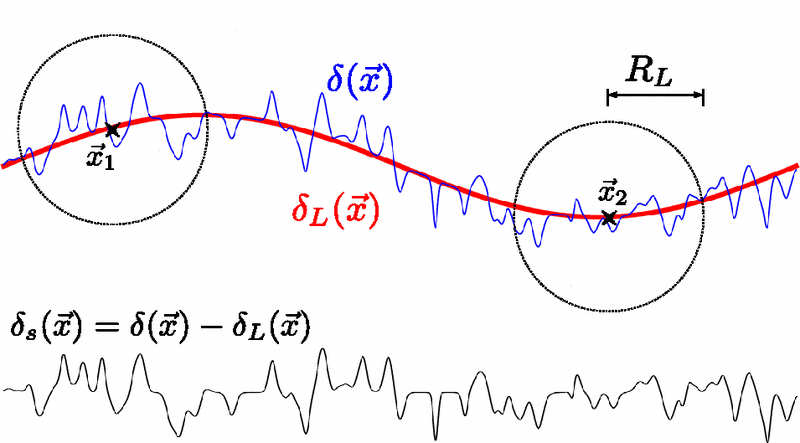
\includegraphics[width=\linewidth]{img/PBS}
	\textcolor{gray}{\fontsize{5.5}{10}\selectfont Image credit: \href{https://link.aps.org/accepted/10.1103/PhysRevD.88.023515}{F. Schmidt, et al.}}	
}
\begin{align*}
	\uncover<+->{
		&\delta(\vec{x}) \equiv \delta_L(\vec{x}) + \delta_s(\vec{x})
		\uncover<2->{,\quad\delta(\vec{x}) = \frac{\rho(\vec{x}) - \rho_c}{\rho_c}}\\~\\
	}
	\uncover<4->{
		&\delta_L(\vec{x}; R_L) = \int \der^2 \vec{x}^\prime \delta(\vec{x}) W_L(\vec{x} + \vec{x}^\prime; R_L)
	}
\end{align*}
\end{column}
\begin{column}{0.5\linewidth}
\centering
\uncover<5->{
	\vskip 10pt
	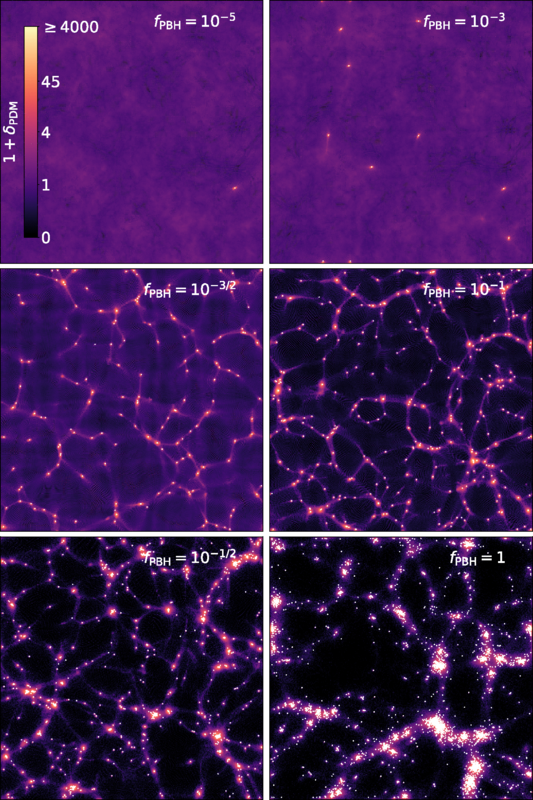
\includegraphics[height=.86\textheight]{img/PBH_Nbody}\\
	\textcolor{gray}{\fontsize{5.5}{10}\selectfont Image credit: \href{https://journals.aps.org/prd/abstract/10.1103/PhysRevD.100.083528}{D. Inman, et al.}}
}
\end{column}
\end{columns}
\end{frame}

